% Section content template for individual Educative lessons
% This file contains the actual content for a specific section
% Generated from Educative API section content

% Section: Sequence Diagram for the ATM System
% Section ID: 4871817715253248
% Section Slug: sequence-diagram-for-the-atm-system
% Generated: 2025-12-12T15:53:59.531782

A sequence diagram is a great way to understand the interactions between different entities and objects in the system. We can create different sequence diagrams for our ATM. For the sake of this lesson, we will create sequence diagrams for balance inquiry from the ATM.

\subsection{Balance inquiry}\label{big_wh-U2Nlmtt5ghxgtf}
\\
The sequence diagram for how to complete the balance inquiry using an ATM should have the following actors and objects that will interact with each other:

\subsubsection{Actors and Objects}\label{peSSJMXPDoU2-c1QKH_qi}

\begin{itemize}
\item
\protect\phantomsection\label{qHi5YcXC9piM8WjnzcZZd}
\textbf{Actor:} User (the person using the ATM)
\item
\protect\phantomsection\label{2JuYtAHjx7IlOCLeZ1R3h}
\textbf{Objects:} ATM, Card issuer (Bank), and Printer
\end{itemize}
\\
\textbf{Steps for balance inquiry using an ATM:}

\begin{enumerate}
\item
\protect\phantomsection\label{enrHp1xHLL6VM1Ptn5ljD}
The user inserts their ATM card into the ATM.
\item
\protect\phantomsection\label{8NDMh1P89W87NW98vhOWA}
The user enters their PIN on the ATM.

\begin{enumerate}
\item
The ATM receives the entered PIN and sends a verification request to the card issuer (Bank).
\end{enumerate}
\item
\protect\phantomsection\label{niW7EHbFnzWg3iPIAAPSH}
The card issuer (Bank) verifies the PIN:

\begin{enumerate}
\item
If the PIN is valid, the Bank notifies the ATM that verification was successful.
\item
If the PIN is invalid, the Bank notifies the ATM, which returns the card to the user, ending the session.
\end{enumerate}
\item
\protect\phantomsection\label{Sjne6lv0jYdRiFuJSqOYc}
If the PIN is verified:

\begin{enumerate}
\item
The user selects the ``Balance Inquiry'' operation on the ATM.
\item
The ATM requests the card issuer (Bank) to retrieve the account balance.
\item
The Bank returns the balance information to the ATM.
\item
The ATM displays the balance to the user.
\item
The user requests a printed receipt (optional).

\begin{enumerate}
\item
If the user requests a receipt, the ATM instructs the Printer to print the balance details, and the receipt is dispensed to the user.
\end{enumerate}
\end{enumerate}
\item
\protect\phantomsection\label{5wTI9L3J9mtANOD3cCxMH}
The user ends the session:

\begin{enumerate}
\item
The ATM returns the card to the user.
\end{enumerate}
\end{enumerate}
\\
This sequence diagram demonstrates the interactions and method calls between the User, ATM, Bank, and Printer during a balance inquiry transaction.

\begin{figure}[htbp]
 \centering
 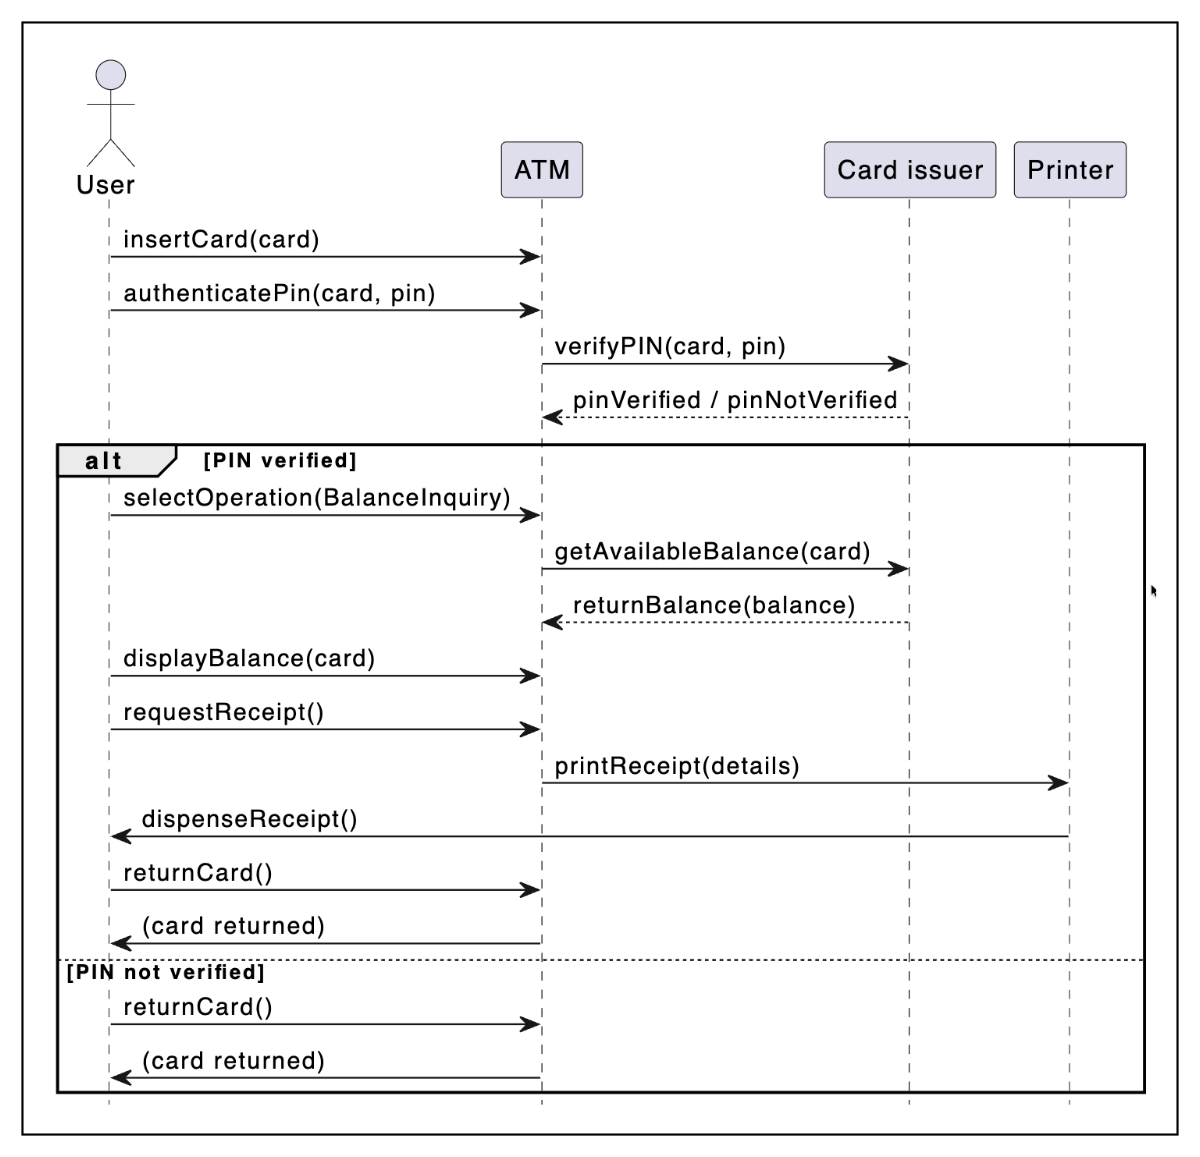
\includegraphics[width=0.5\textwidth]{Images/chapter_16/section_4871817715253248/4522054924500992.png}
 \caption{The sequence diagram for how to complete a balance inquiry from an ATM}
\end{figure}

In the next lesson, we will create activity diagrams for the ATM.

% End of section content